\documentclass[mathserif,serif]{beamer}
\usepackage[utf8]{inputenc}
\usepackage[english]{babel}
\usepackage{amsmath}
\usepackage{stmaryrd}
\usepackage{amsfonts}
\usepackage{amssymb}
\usepackage{hyperref}
\usepackage{graphicx}
\usepackage{url}
\usepackage{amsthm}
\usepackage{mathpartir}
\usepackage{listings}
\usetheme{Warsaw}

\lstset{
	basicstyle=\ttfamily\small,
	mathescape=false,
	frame=single,
	keywordstyle=\color{blue},
	breaklines=true
	showstringspaces=false}

\begin{document}

\newtheorem{proposition}{Proposition}
\setbeamertemplate{theorems}[numbered]

\author[Di Giacomo]
{Francesco ~Di Giacomo}
\institute[Universities Here and There] % (optional)
{
  Università Ca' Foscari di Venezia - PhD in Computer Science
}
\date{}
\title{Building Domain Specific Languages with the Metacasanova meta-compiler}

\frame{\titlepage}

\begin{frame}
	\frametitle{Introduction}
	\framesubtitle{Importance of domain specific languages}
	\begin{itemize}
		\item They allow to express the solution of a problem in a more natural way.
		\item They provide constructs that are domain-specific not provided by GPL's.
		\item They allow to develop complete application programs for a specific domain more quickly.
	\end{itemize}
	
	\pause
	\textbf{CONSEQUENCE:} It is desirable to deploy a DSL's when the scope of the application is very specific.
	
\end{frame}

\begin{frame}
	\frametitle{Introduction}
	\framesubtitle{Some DSL's examples}
	
	\begin{figure}
		\centering
		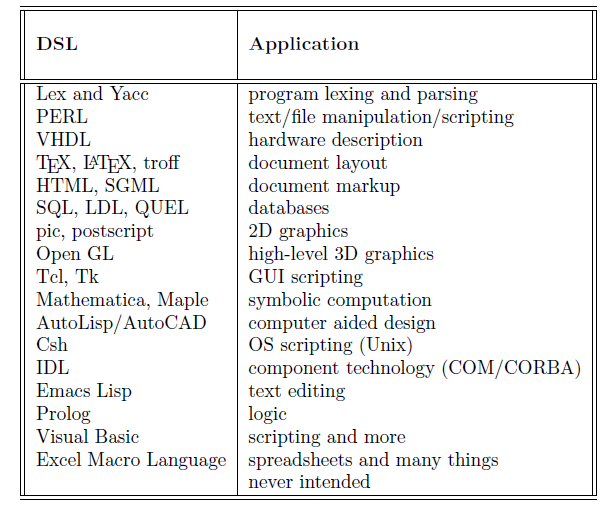
\includegraphics[scale=0.5]{Figures/dsl_table}
	\end{figure}	
\end{frame}

\begin{frame}
	\frametitle{Introduction}
	\framesubtitle{Disadvantages of DSL's}
	
	\textbf{PROBLEM}: Creating DSL's requires to implement a compiler/interpreter for the language.
	
	\begin{itemize}
		\item Compilers are complex
		\item Several modules: parser, type checker, code generator/code interpreter
		\item Require a lot of development time.
		\item Not flexible: adding features to the language compiled by hard-coded compilers takes a considerable effort.
	\end{itemize}
\end{frame}

\begin{frame}
	\frametitle{Towards meta-compilers}
	\framesubtitle{Implementing compilers is repetitive}
	
	The implementation of the compiler is a repetitive process:
	\begin{itemize}
		\item The parser can be created with parser generators (e.g. Yacc)
		\item The type system must be implemented in the host language.
		\item The operational semantics must be reflected in the generated code (code generations).
	\end{itemize}
\end{frame}

\begin{frame}
	\frametitle{Towards meta-compilers}
	\framesubtitle{Type system and semantics}
	
	How they are formalized:
	\begin{itemize}
		\item Expressed in a form that mimics logical rules.
		\item They are compact.
		\item They are readable.
	\end{itemize}
	
	How they are implemented:
	\begin{itemize}
		\item Encoded with the abstractions provided by the host language.
		\item Readability is usually lost in the translation process.
		\item The effort required for the translation is high.
	\end{itemize}
	
\end{frame}

\begin{frame}
	\frametitle{Towards meta-compilers}
	\framesubtitle{Example of semantics}
	
	Semantics of a statement that waits ford a condition or a certain amount of seconds:
	
	\vspace{0.5cm}
	\small
	\inferrule
	{\langle t - dt > 0 \rangle \; \Rightarrow \; \texttt{true}}
	{\langle \mathtt{wait} \; t;k \; dt \rangle \; \Rightarrow \; \langle \mathtt{wait} \; t - dt ; k \; dt \rangle}
	
	\inferrule
	{\langle t - dt > 0 \rangle \; \Rightarrow \; \texttt{false}}
	{\langle \mathtt{wait} \; t ; k \; dt \rangle \; \Rightarrow \; \langle k \; dt \rangle}
	
	\small
	\inferrule
	{\langle c \rangle \; \Rightarrow \; \mathtt{true}}
	{\langle \mathtt{wait} \; c;k \; dt \rangle \; \Rightarrow \; \langle k \; dt\rangle}
	
	\inferrule
	{\langle c \rangle \; \Rightarrow \; \mathtt{false}}
	{\langle \mathtt{wait} \; c;k \; dt \rangle \; \Rightarrow \; \langle \mathtt{wait} \; c;k \; dt \rangle}
\end{frame}

\begin{frame}
	\frametitle{Towrds meta-compilers}
	\framesubtitle{Implementation of the semantics}
	
	\begin{figure}
		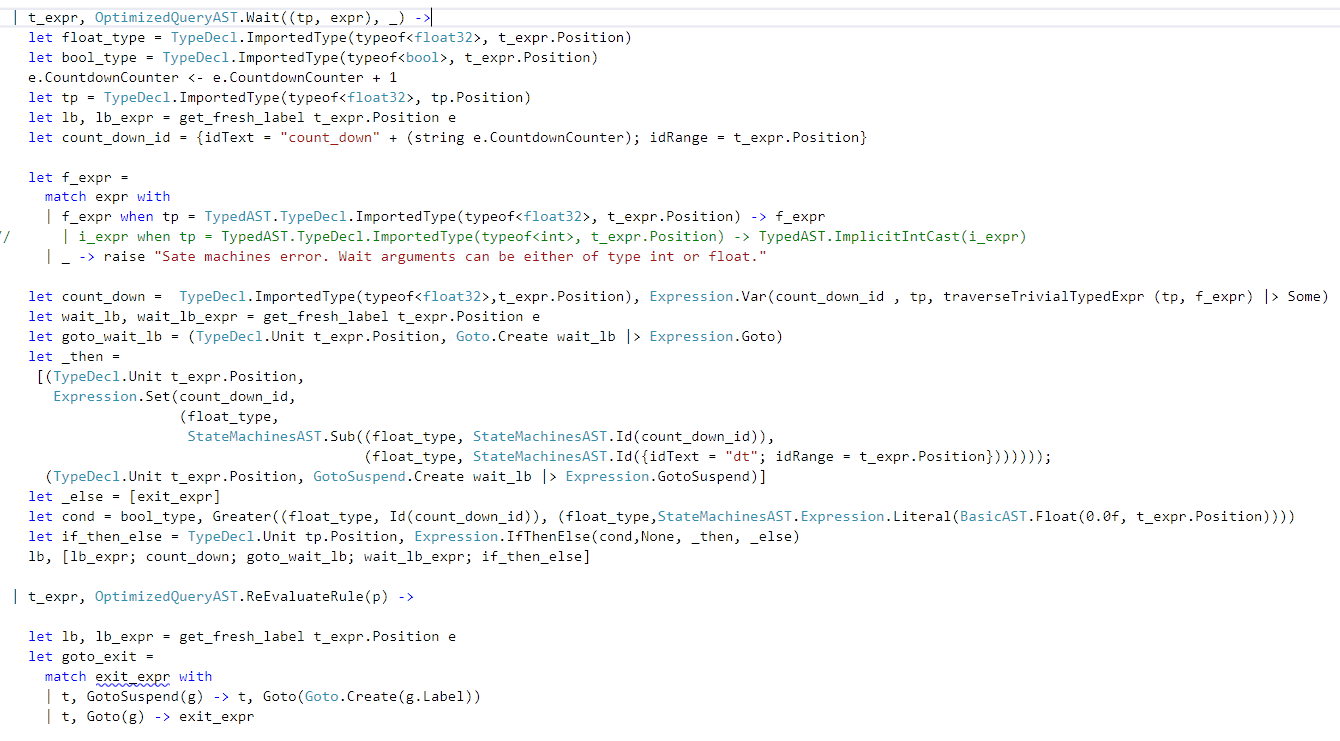
\includegraphics[scale=0.4]{Figures/wait_code}
	\end{figure}
\end{frame}

\begin{frame}
	\frametitle{Towards meta-compilers}
	\framesubtitle{Observations}
	
	\begin{itemize}
		\item Formal semantics provide a clear, compact, and simple way to describe the constructs of the language.
		\item Implementing a compiler in a GPL requires to encode the semantics within the abstractions provided by it.
		\item The result is something completely different.
	\end{itemize}
\end{frame}

\begin{frame}
	\frametitle{Towards meta-compilers}
	\framesubtitle{Idea}
	
	\large
	\color{red}
	Why not implementing a program that can take as input the language definition expressed in the fashion of the semantics rules, a program written in that language, and outputs executable code?

	\pause
	
	\vspace{1cm}
	\color{black}
	We can: this software is defined as meta-compiler.
\end{frame}

\begin{frame}
	\frametitle{Meta-casanova}
	\framesubtitle{General overview}
	
	\begin{itemize}
		\item Metacasanova is a metacompiler that uses semantics rules to define a language.
		\item A program in Meta-casanova contains:
		\begin{itemize}
			\item Data declarations
			\item Function declarations
			\item Subtypes declarations
			\item Rules
		\end{itemize}
	\end{itemize}

\end{frame}

\begin{frame}[fragile]
	\frametitle{Meta-casanova}
	\framesubtitle{Data definition example}
	
	Below the code for:
	\begin{itemize}
		\item Integer constant
		\item Sum of arithmetic expressions
		\item While loop
	\end{itemize}
	
	\begin{lstlisting}
Data "$i" -> <<int>> : Value Priority 300
Data Expr -> "+" -> Expr : Expr Priority 100
Data "while" -> Expr -> Expr : Expr Priority 10
	\end{lstlisting}
\end{frame}

\begin{frame}[fragile]
	\frametitle{Meta-casanova}
	\framesubtitle{Function definition example}
	Below the code for:
	\begin{itemize}
		\item Declaration of evaluation of expressions.
		\item Function to add a variable to the symbol table.
	\end{itemize}
	
	\begin{lstlisting}
Func "eval" -> Expr : RuntimeOp => EvaluationResult Priority 0
Func SymbolTable -> "defineVariable" -> Id : MemoryOp => SymbolTable Priority 300
	\end{lstlisting}
\end{frame}

\begin{frame}[fragile]
	\frametitle{Meta-casanova}
	\framesubtitle{Subtyping example}
	
	In the code below we declare that a value, id, and a sequence of expressions are considered expressions as well.
		\begin{lstlisting}
Value is Expr
Id is Expr
ExprList is Expr
		\end{lstlisting}
\end{frame}

\begin{frame}
	\frametitle{Meta-casanova}
	\framesubtitle{Rules}
	
	\begin{itemize}
		\item A rule is made of a set of premises and a conclusion. A premise can be a function call or a predicate.
		\item First the left part of the conclusion is evaluated. 
		\item The language does pattern matching on the function arguments and if it fails the rule is not executed.
		\item The premises are evaluated in order. The language looks for possible candidate rules for the execution, i.e. rules containing in the conclusion the function called by the premise. In case of predicates, the predicate is immediately evaluated.
		\item If the rule call fails, then the entire rule evaluation fails.
	\end{itemize}
\end{frame}

\begin{frame}
	\frametitle{Meta-casanova}
	\framesubtitle{Semantics of rule evaluation}
	
	Consider:
	\begin{itemize}
		\item A set of rules $R$.
		\item A set of function calls $F$ for each rule in $R$.
		\item A set of clauses $C$ for each rule in $R$.
		\item The notation $f^{r}$ means apply the function $f$ through the rule $r$.
		\item The notation  $\langle f^{r} \rangle$ means evaluating the application of $f$ through $r$.
		\item The result of a rule is in general a set because it is possible to allow the rule to branch, i.e. if the evaluation of a premise succeeds by using more than one rule, we return all the possible result.
	\end{itemize}
\end{frame}

\begin{frame}
	\frametitle{Meta-casanova}
	\framesubtitle{Semantics of rule evaluation}
	
	\begin{mathpar}
		\mprset{flushleft}
		\inferrule*[left=R1:]
		{C = \emptyset \\\\ F = \emptyset}
		{\langle f^{r} \rangle \Rightarrow \lbrace x \rbrace} \\
		
		\mprset{flushleft}
		\inferrule*[left=R2:]
		{\forall c_{i} \in C \;, \langle c_{i} \rangle \Rightarrow true \\\\
			\forall f_{j} \in F \; \exists r_{k} \in R \; | \; \langle f_{j}^{r_{k}} \rangle \Rightarrow \lbrace x_{k_{1}}, x_{k_{2}}, ..., x_{k_{m}} \rbrace}
		{\langle f^{r} \rangle \Rightarrow \lbrace x_{1}, x_{2}, ..., x_{n} \rbrace} \\
		
		\mprset{flushleft}
		\inferrule*[left=R3(a):]
		{\exists c_{i} \in C \; | \; \langle c_{i} \rangle \Rightarrow false}
		{\langle f^{r} \rangle \Rightarrow \emptyset} \\
		
		\mprset{flushleft}
		\inferrule*[left=R3(b)]
		{\forall r_{k} \in R \; \exists f_{j} \in F \; | \; \langle f_{j}^{r_{k}} \rangle \Rightarrow \emptyset}
		{\langle f^{r} \rangle \Rightarrow \emptyset}
	\end{mathpar}
\end{frame}

\begin{frame}[fragile]
	\frametitle{Meta-casanova}
	\framesubtitle{Rules - Example}
	
	\begin{lstlisting}
---------------------
eval ($i v) => ($i v)
	\end{lstlisting}
	
	\begin{itemize}
		\item The rule above does not contain premises, i.e. it is an axiom.
		\item If the pattern matching on the conclusion succeeds, i.e. the input is an integer constant, then we simply return the constant as evaluation of the expression.
	\end{itemize}

\end{frame}

\begin{frame}[fragile]
	\frametitle{Meta-casanova}
	\framesubtitle{Rules - Example}
	
		\begin{lstlisting}
eval expr1 => ($i val1)
eval expr2 => ($i val2)
<<val1 + val2>> => arithmeticResult
---------------------------------
eval expr1 + expr2 => $i arithmeticResult


	\end{lstlisting}
	
	\begin{itemize}
		\item The first rule does pattern matching on \texttt{expr1 + expr2}. This means that if the input is not in that form, the rule is not triggered.
		\item In the premises, if the result of the recursive call to the evaluation function is not an integer constant, the rule evaluation fails. This might happen when executing, for example, the sum of two strings.
		\item The third premises emits C\# code to do the sum computation.
		\item The result is another integer constant containing the sum of the two expressions.
		\item The second rule is an axiom: if the expression is an integer constant we simply return it.
	\end{itemize}

\end{frame}

\begin{frame}
	\frametitle{Case study: Casanova 2.5}
	
	\begin{itemize}
		\item \textbf{Entities:} They contain both the data and the behaviour of the objects in the game
		\item \textbf{Rules:} They define the behaviour of the entity. Once a rule ends its execution it is restarted at the next frame.
		\item \textbf{Domain:} A set of entity attributes the rule is allowed to change. A rule can always read all fields but can modify only those in the domain through a \texttt{yield} statement.
	\end{itemize}
\end{frame}

\begin{frame}[fragile]
	\frametitle{Example of program in Casanova}
	\begin{lstlisting}[basicstyle = \ttfamily\small]
entity Guard = {
Position  : Vector2
Velocity  : Vector2

rule Position = Position + Velocity * dt

rule Velocity =
wait Position.X >= 300f || Position.X <= 0f
yield new Vector2(-Velocity.X, 0f)
}
	\end{lstlisting}
\end{frame}

\begin{frame}
	\frametitle{Rule pausing}
	Rule execution can be paused with built-in statements:
	\begin{itemize}
		\item \texttt{wait} takes either a floating point value or a predicate. In the first version the rule is paused by the given amount of seconds, in the second it is paused until the condition is met.
		\item \texttt{yield} updates the fields in the domain with the given values. The rule execution is paused by one frame in order to be able to see the changes at the next game update.
	\end{itemize}
\end{frame}

\begin{frame}
	\frametitle{Semantics of wait}
	\begin{mathpar}
		\small
		\inferrule
		{\langle t - dt > 0 \rangle \; \Rightarrow \; \texttt{true}}
		{\langle \mathtt{wait} \; t;k \; dt \rangle \; \Rightarrow \; \langle \mathtt{wait} \; t - dt ; k \; dt \rangle}
		
		\inferrule
		{\langle t - dt > 0 \rangle \; \Rightarrow \; \texttt{false}}
		{\langle \mathtt{wait} \; t ; k \; dt \rangle \; \Rightarrow \; \langle k \; dt \rangle}
		
		\small
		\inferrule
		{\langle c \rangle \; \Rightarrow \; \mathtt{true}}
		{\langle \mathtt{wait} \; c;k \; dt \rangle \; \Rightarrow \; \langle k \; dt\rangle}
		
		\inferrule
		{\langle c \rangle \; \Rightarrow \; \mathtt{false}}
		{\langle \mathtt{wait} \; c;k \; dt \rangle \; \Rightarrow \; \langle \mathtt{wait} \; c;k \; dt \rangle}
	\end{mathpar}
\end{frame}

\begin{frame}[fragile]
	\frametitle{Implementation of wait in Metacasanova}
	In the following waiting on a condition is called \texttt{when} because Metacasanova does not currently support operators overloading
	\begin{lstlisting}[basicstyle=\ttfamily\tiny]
eval expr ctxt => ($f t)
<<t <= dt>> == false
----------------------------------
eval_s (wait expr) k ctxt dt => Suspend (wait $f (<<t - dt>>));k ctxt

eval expr ctxt => ($f t)
<<t <= dt>> == true
----------------------------------
eval_s (wait expr) k ctxt dt => Resume k ctxt


eval expr ctxt => ($b true)
---------------------------------------------
eval_s (when expr) k ctxt dt => Atomic k ctxt

eval expr ctxt => ($b false)
------------------------------------------
eval_s (when expr) k ctxt dt => Suspend (when expr);k ctxt
	\end{lstlisting}
	
\end{frame}

\begin{frame}
	\frametitle{Results: patrol script}
	\begin{itemize}
		\item Script making a guard patrol two checkpoints
		\item Tests run with the script written in Casanova 2.5 and Python.
		\item Implementation of Casanova 2.5 compared with the code length of the hard-coded compiler modules for Casanova 2.0.
		\item Python is used as a scripting language in several games (e.g. World in Conflict, Civilization IV).
		\item We neglected C\# because we already have benchmarks for that in Casanova 2.0 and both languages are faster of several orders of magnitude.
	\end{itemize}
\end{frame}

\begin{frame}
	\frametitle{Results: patrol script}
	\begin{table}
		\centering
		\tiny	
		\begin{tabular}{|c|c|c|}
			\hline
			\multicolumn{3}{|c|}{\textbf{Casanova 2.5}} \\
			\hline
			Entity \# & Average update time (ms) & Frame rate \\
			\hline
			100 & 0.00349 & 286.53 \\
			\hline
			250 & 0.00911 & 109.77 \\
			\hline
			500 & 0.01716 & 58.275 \\
			\hline
			750 & 0.02597 & 38.506 \\
			\hline
			1000 & 0.03527 & 28.353 \\
			\hline
			\multicolumn{3}{|c|}{\textbf{Python}} \\
			\hline
			Entity \# & Average update time (ms) & Frame rate \\
			\hline
			100 & 0.00132 & 756.37 \\
			\hline
			250 & 0.00342 & 292.05 \\
			\hline
			500 & 0.00678 & 147.54 \\
			\hline
			750 & 0.01087 & 91.988 \\
			\hline
			1000 & 0.01408 & 71.002 \\
			\hline
		\end{tabular}
		\caption{Patrol sample evaluation}
		\label{tab:evaluation}
	\end{table}	
\end{frame}

\begin{frame}
	\frametitle{Results: patrol script}
	\begin{table}
		\centering
		\tiny	
		\begin{tabular}{|c|c|}
			\hline
			\multicolumn{2}{|c|}{\textbf{Casanova 2.5 with Metacasanova}} \\
			\hline
			Module & Code lines \\
			\hline
			Data structures and function definitions & 40 \\
			\hline
			Query Evaluation & 16 \\
			\hline
			While loop & 4 \\
			\hline
			For loop & 5 \\
			\hline
			If-then-else & 4 \\
			\hline
			When & 4 \\
			\hline
			Wait & 6 \\
			\hline
			Yield & 10 \\
			\hline
			Additional rules for Casanova program evaluation & 40 \\
			\hline
			Additional rules for basic expression evaluation & 201 \\
			\hline
			\multicolumn{2}{|l|}{\textbf{Total: } 300} \\
			\hline
			\multicolumn{2}{|c|}{\textbf{Casanova 2.0 compiler}} \\
			\hline
			Module & Code lines \\
			\hline
			While loop & 10 \\
			\hline
			For-loop and query evaluation & 44 \\
			\hline
			If-Then-Else & 15 \\
			\hline
			When & 11 \\
			\hline
			Wait & 24 \\
			\hline
			Yield & 29 \\
			\hline
			Additional structures for rule evaluation & 63 \\
			\hline
			Structures for state machine generations & 754 \\
			\hline
			Code generation & 530 \\
			\hline
			\multicolumn{2}{|l|}{\textbf{Total: } 1480} \\
			\hline			
		\end{tabular}
		\caption{Metacasanova vs Casanova 2.0 compiler}
		\label{tab:evaluation}
	\end{table}	
\end{frame}

\begin{frame}
	\frametitle{Conclusion}
	\textbf{Advantages:}
	\begin{itemize}
		\item The code length to define the semantics of the language is almost 5 times shorter.
		\item Using Metacasanova greatly reduces the effort to build a compiler.
		\item The definition of the language in Metacasanova is almost identical to the formal definition.
		\item Extending the language becomes easier.
	\end{itemize}
	\textbf{Disadvantages:}
	\begin{itemize}
		\item The generated code is slower than Python but of the same order of magnitude.
		\item Code performance affected by maps used to model the memory.
		\item The code generation requires further improvement.
		\item Using data structures and methods from external libraries requires to build a wrapper with meta-types and meta-functions.
	\end{itemize}
\end{frame}

\begin{frame}
	\frametitle{Related work}
	
	\begin{itemize}
		\item META II family languages, parser generators plus code generators. Untyped. (1970's).
		\item RML language family based on natural semantics (1996). It generates C code.
	\end{itemize}
\end{frame}

\begin{frame}
	\frametitle{Future work}
	
	\begin{itemize}
		\item Type classes and inliner to access fields in records by using the result of type function calls.
		\item Handling imported libraries automatically by generating \texttt{unsafe} type to handle side effects, or allow the programmer to specify a mapping to metacompiler types.
		\item Expand Casanova 2.5 with networking primitives.
	\end{itemize}
\end{frame}

\begin{frame}
	\centering
	\Huge
	Tank you!\\
	\vspace{0.5cm}
	\textcolor{red}{Questions?}
\end{frame}

\end{document}